\chapter{Signal Model and Generation}
\label{sec:Samples/Signal}

We generate MC events to simulate all 27 production and decay mode combinations (see Sec.~\ref{sec:Introduction}). Generation for the model begins with a FeynRules Model file \cite{SeesawIII_Biggio}. Monte Carlo events are then generated in MadGraph5\_aMC@NLO \cite{Alwall:2011uj}. Bosonic decays are handled through Pythia 8, which is also in charge of hadronization \cite{Sjostrand:2007gs}. At the analysis level, we apply weights to correct for mismodeling of pile-up and \MET resolution.

The production cross sections were calculated with NLO + NLL accuracy using the CTEQ6.6 and MSTW2008nlo90cl parton distribution functions (PDFs) \cite{Fuks:2012qx,Fuks:2013vua}. Flavor-democratic values of the mixing angles are taken ($V_e = V_\mu = V_\tau = 10^{-6}$). This has no direct consequence on the fermion production cross section, but affects the branching ratios. The branching fraction of a heavy fermion to a lepton of flavor $\ell = e, \mu, \tau$ is proportional to $v_{\ell N} = \frac{V_\ell}{\sqrt{|V_e|^2 + |V_\mu|^2 + |V_\tau|^2}}$. Therefore, the flavor-democratic scenario gives $v_{\ell N} = \frac{1}{\sqrt{3}}$. The branching ratios from the pair-produced fermions to the bosonic level of the most relevant decay modes are given in Fig.~\ref{fig:SeesawBR}.

\begin{figure}
\begin{center}
	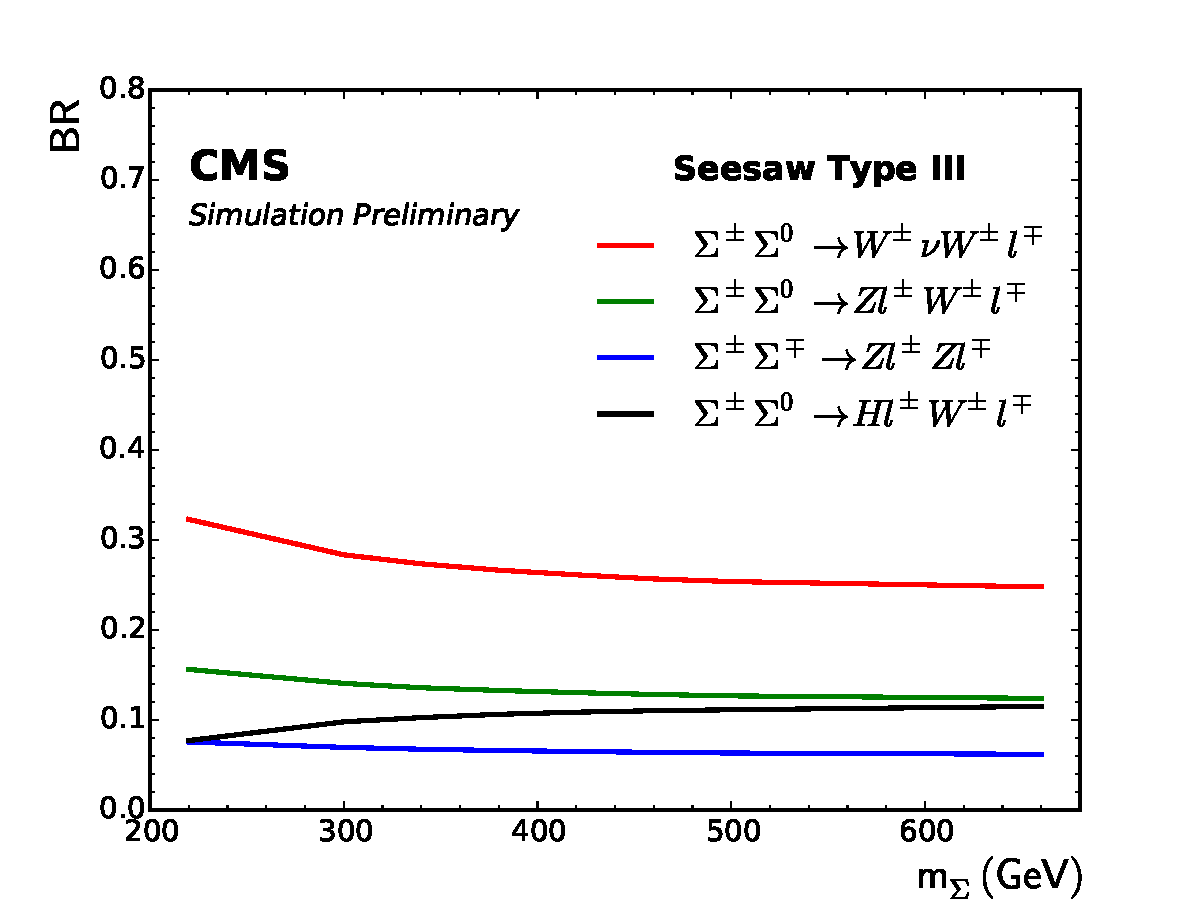
\includegraphics[width=.8\textwidth]{SignalModel/BR}
	\caption{Branching ratios from the pair-produced fermions to the bosonic level of the most relevant decay modes.
	\label{fig:SeesawBR}}
\end{center}
\end{figure}
